\section{General-Purpose Counterfactuals}
\label{sec:general_purpose}



\newcommand{\tagdefine}[1]{\emph{{\color{darkgray}#1} }}
%\renewcommand{\arraystretch}{1.1}
\newcommand{\TagTable}{
\begin{table*}
\small
\centering
\begin{tabular}{@{} p{0.11\linewidth} p{0.61\linewidth} p{0.22\linewidth} @{}}
\toprule
\textbf{\Tagstr} & \textbf{Definitions and \sysname-generated Examples} & \textbf{Training Datasets} \\ 
\midrule
\ctrltag{negation}
 & A dog is \add{not} embraced by the woman.
 &\cite{kaushik2019learning}
\\ \midrule
\ctrltag{quantifier}
 & \swap{A dog is}{Three dogs are} embraced by the woman. 
 &\cite{gardner2020contrast}
\\ \midrule
\ctrltag{shuffle}
 & \tagdefine{To move (or swap) key phrases or entities around the sentence.} \newline
 A \swap{dog}{woman} is embraced by the \swap{woman}{dog}.
 &\cite{zhang2019paws}
\\ \midrule
\ctrltag{lexical}
 & \tagdefine{To change just one word or noun chunk without altering the POS tags.} \newline
 A dog is \swap{embraced}{attacked} by the woman.
 &\cite{sakaguchi2019winogrande}
\\ \midrule
\ctrltag{resemantic}
 & \tagdefine{To replace short phrases without altering the remaining dependency tree.}\newline
 A dog is \swap{embraced by the woman}{wrapped in a blanket}.
 &\cite{wieting2017paranmt}
\\ \midrule
\ctrltag{insert}
 & \tagdefine{To add short phrases without altering the remaining dependency tree.} \newline
 A dog is embraced by the \add{little} woman.
 &\cite{mccoy2019right}
\\ \midrule
\ctrltag{delete}
 & \tagdefine{To remove short phrases without altering the remaining dependency tree.} \newline
 A dog is embraced \remove{by the woman}.
 &\cite{mccoy2019right}
\\ \midrule
\ctrltag{restructure}
 & \tagdefine{To alter the dependency tree structure, \eg changing from passive to active.} \newline
 A dog is \swap{embraced by}{hugging} the woman.
 &\cite{wieting2017paranmt}
\\
\bottomrule
\end{tabular}
\vspace{-5pt}
\caption{
We design a list of \tagstrs to guide generation.
We show \emph{\sysname-generated} counterfactual examples, and the representative training datasets for each corresponding pattern. 
Details are in Appendix~\ref{appendix:train_data}.
%More examples are in Appendix~\ref{appendix:example}.
}
%\wts{Change all the examples to be on an identical sentence, not all different cases. And consider further annotate the tags based on whether they just do semantic change or also syntactic change.}}
\label{table:ctrltag}
%\vspace{-10pt}
\end{table*}
}
% on a particular instance
% 
\subsection{Definition and Desiderata}
\label{sec:desiderata}


Given an instance $x$, a generator $g$ produces a set of counterfactuals $\hat{\xset} = \{\xp_1, \xp_2, ...\}$ with various relationships $x \veryshortarrow \xp_i$. % (referred as $\relation{\xp_i}$ for simplicity).
% Each $\xp_i$ perturbs $x$ with certain strategies like negations, syntactic restructuring, etc., and the edited spans are instantiations of the strategies.
For example, \swap{great}{not great}, \swap{kids}{no one} in Figure~\ref{fig:teaser}B are both instances of the \ctrltag{negation} relationship.
% The importance of certain $\relation{\xp}$ changes along with applications.
Each $(x, \xp)$ pair shares multiple relationships --- these two are also instances of the \emph{label flipping} relationship if the task is sentiment analysis (but might not be for other tasks).
As illustrated in \S\ref{sec:intro}, knowing which relationships apply aids selection for downstream applications.

We expect $g$ to produce counterfactuals $\xp$ that are (1) \textbf{close} to $x$, preferably only involving the minimal changes necessary to establish a certain effect~\cite{pearl2018causal}, allowing users to make causality assessments.
The generated $\xp$ should also be (2) \textbf{fluent}, \ie grammatically correct~\cite{morris2020textattack} and semantically meaningful (\eg \exinline{Colorless green ideas sleep furiously} is not meaningful~\cite{chomsky2002syntactic}).
Fluency operationalizes ``probable'' counterfactuals in the context of NLP;
as \citet{kahneman} stated, humans strongly favor counterfactuals that are close to the original instance, but also prefer those that could have easily happened without assuming rare events or strange coincidences.
%Humans strongly favor counterfactuals that are close to the original instance, but also prefer them to be probable, \ie they could have easily happened without assuming rare events or strange coincidences~\cite{kahneman}.
%We operationalize ``probable'' in the context of NLP by requiring $g$ to generate (2) \textbf{fluent} $\xp$, \ie grammatically correct~\cite{morris2020textattack} and semantically meaningful (\eg \exinline{Colorless green ideas sleep furiously} is not meaningful~\cite{chomsky2002syntactic}).
Further, as a general-purpose generator, $g$ should produce counterfactuals with a measure of (3) \textbf{control} over relationships $x \veryshortarrow \xp$,  %$\relation{\xp}$,
such that the counterfactuals can vary with the object-of-attention in each application (the ``focus rule''~\cite{kahneman}).
Finally, %even though infinite diverse counterfactuals can be produced~\cite{pearl2018causal},
we expect $g$ to output a (4) \textbf{diverse} set of $\xp$ in terms of relationships, covering a large variety of ``what-ifs'' for different applications~\cite{pearl2018causal}.


\TagTable


\begin{figure}[t]
\centering
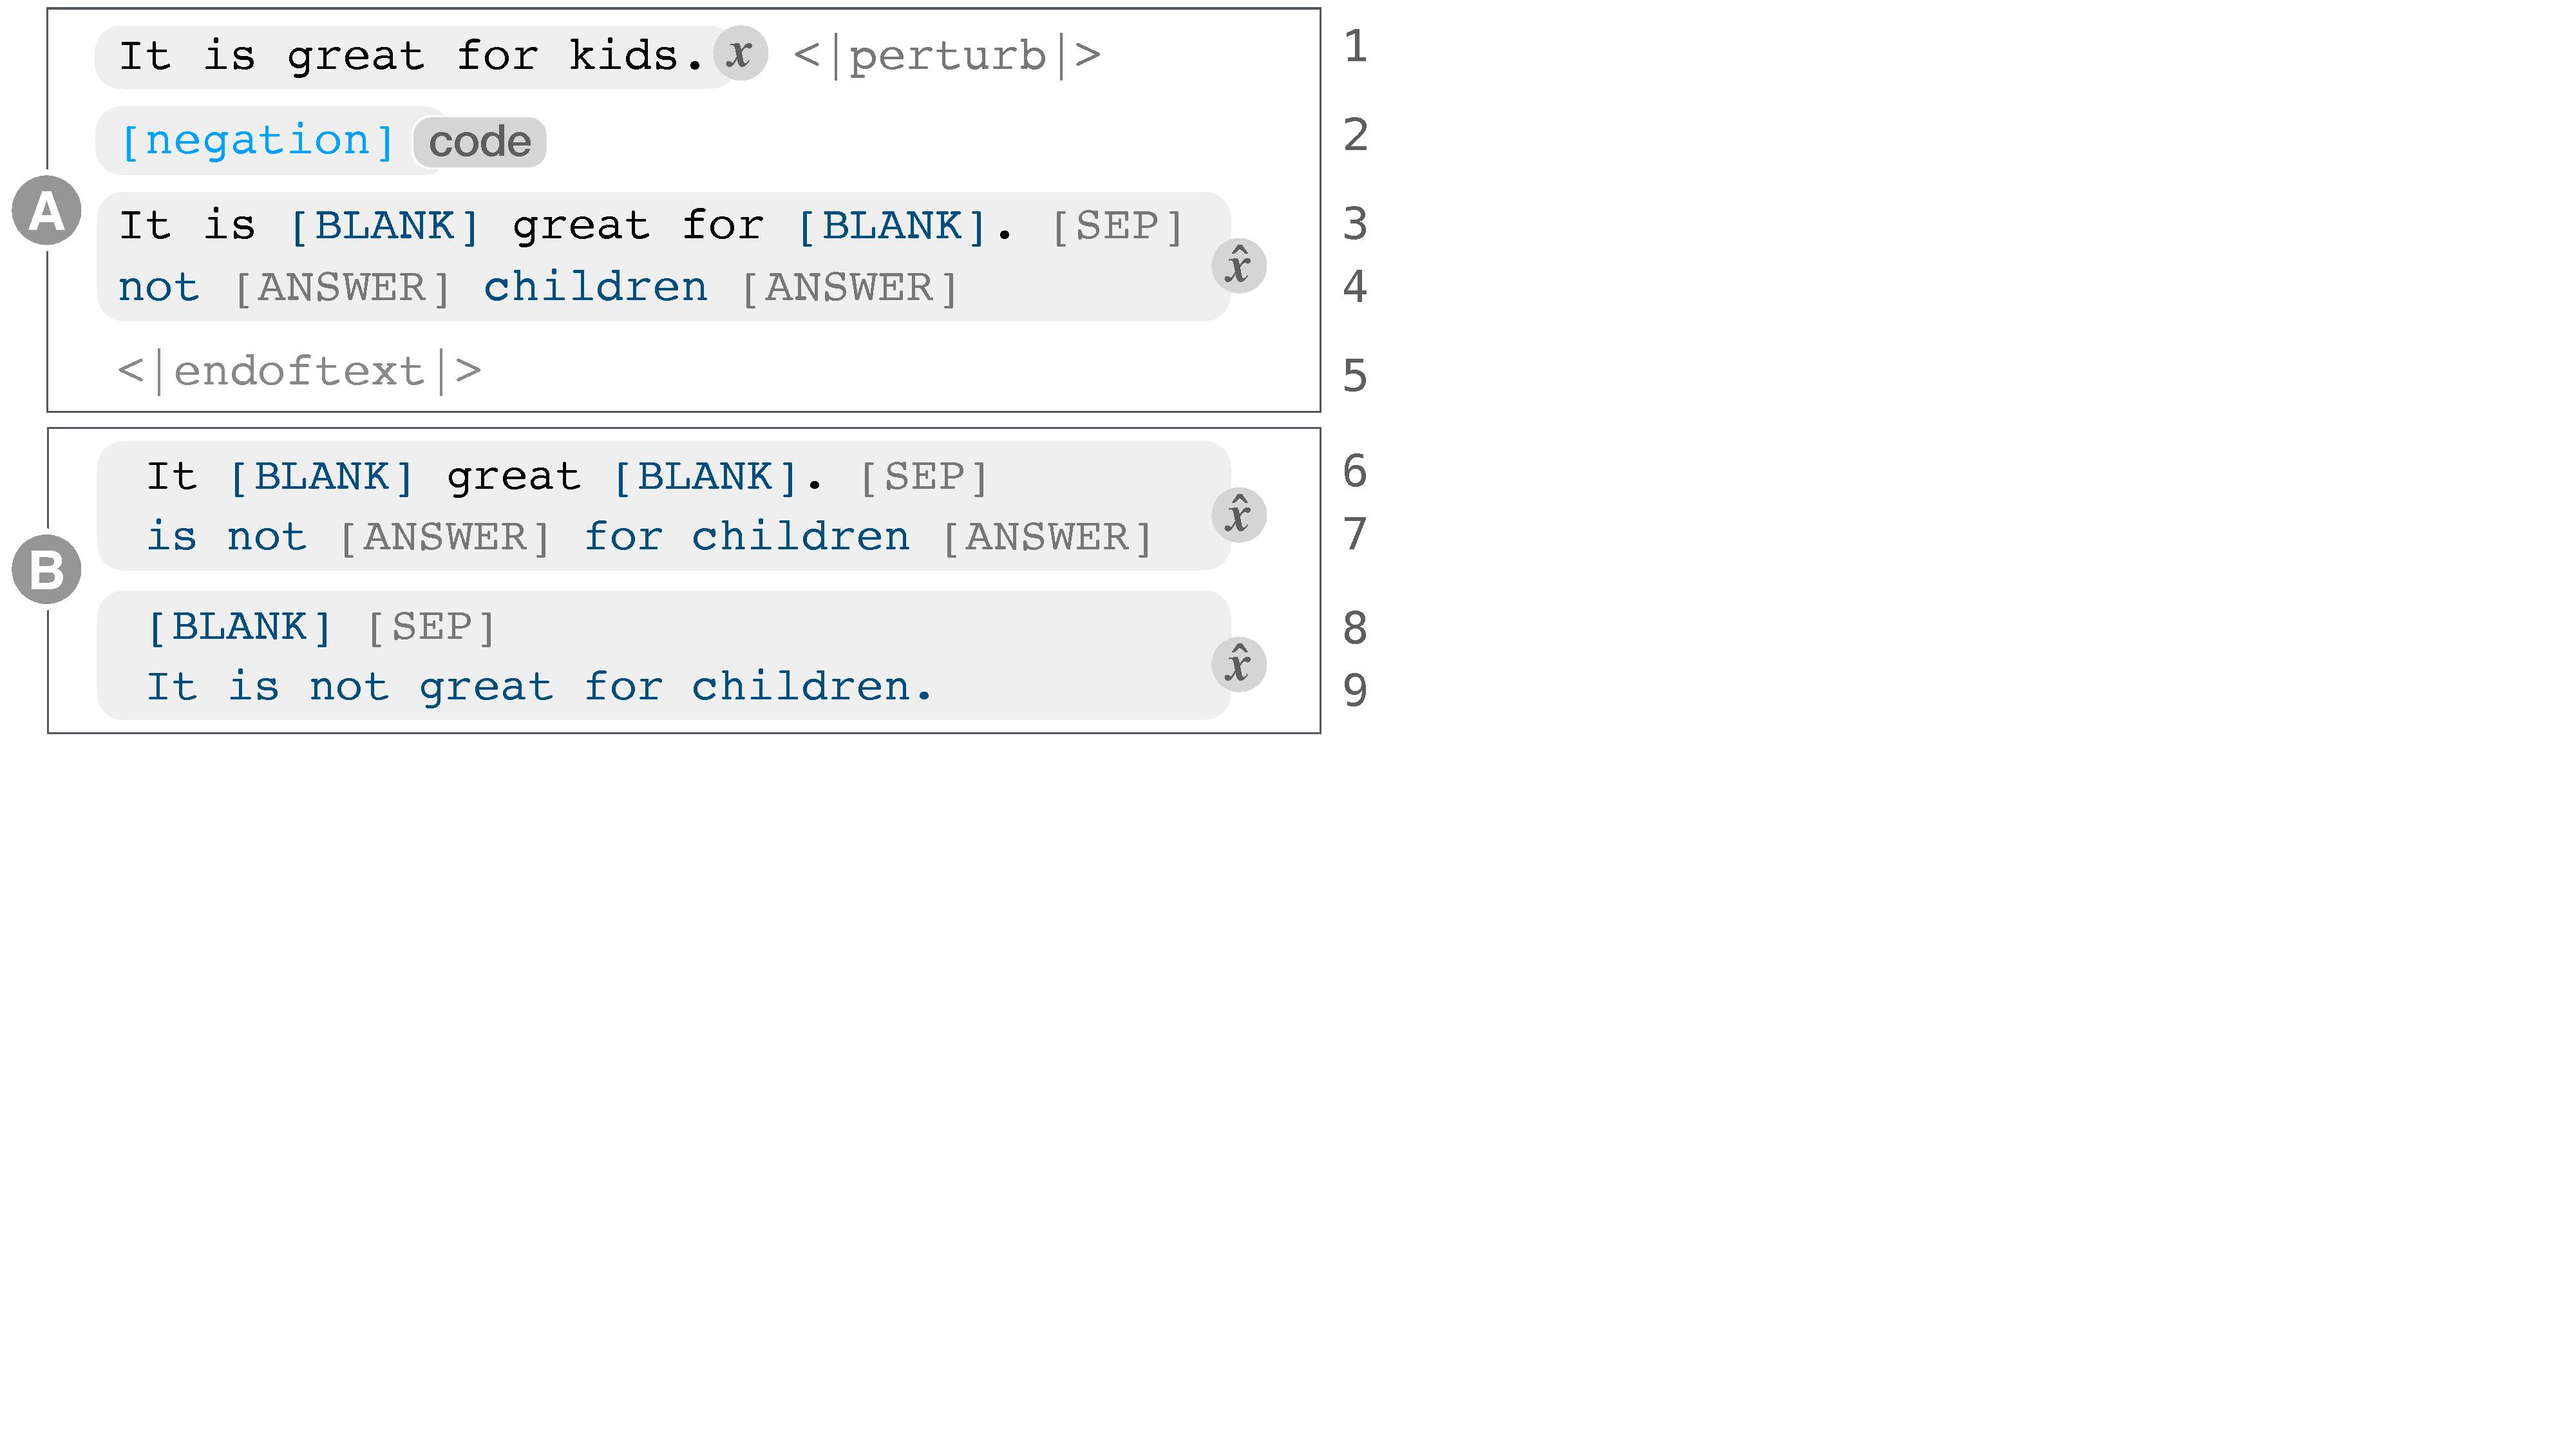
\includegraphics[trim={0 18.6cm 31.5cm 0cm}, clip, width=1\columnwidth]{figures/blank.pdf}
\vspace{-15pt}
\caption{ 
(A) \sysname prompt format, which concatenates the original $x$, the \tagstr, and the $\xp$ (\exinline{It is not great for children} converted to an infilling structure).
At \emph{generation} time, \sysname accepts prompts that just include $x$ (Line 1), or optionally with the \tagstrshort and the \texttt{[BLANK]}s (Lines 2--3), and fills in the blanks sequentially with spans separated by \texttt{[ANSWER]}s (Line 4).
%During training, the \tagstrshorts and blanks are automatically extracted.
(B) \sysname allows blanking at different granularities (even the entire sentence), such that Lines 3--4 in (A) can be replaced by Lines 6--7 or 8--9. 
%\dq{}
%We get multiple training texts per pair, by blanking $\xp$ subtrees that contain the change, or the entire sentence.
}
\vspace{-10pt}
\label{fig:blank}
\end{figure}


\subsection{Conditional Counterfactual Generation}
\label{subsec:nlg}




%We frame counterfactual generation as a conditional text generation task using language models (LMs).
We frame counterfactual generation as a conditional text generation task using language models (LMs)\fixed{, and train \sysname by finetuning GPT-2~\cite{radford2019language} using the following prompt design (alternative LMs could also have been used).}


\paragraph{\fixed{Prompt format design.}}
To ensure that $\xp$ is \emph{close} to $x$ rather than arbitrary text, we condition the generation on $x$, followed by a special token (Line 1 in Figure~\ref{fig:blank}A).
In Line 2, we have \emph{\tagstrs} \cite{ctrl} such as \ctrltag{negation}.
We design them to specify types of perturbation from among lexical, syntactic, or semantic aspects (see Table \ref{table:ctrltag}), inspired by prior work that categorizes manually created counterfactuals~\cite{kaushik2019learning, gardner2020contrast}.
% All the \tagstrshorts are described in Table~\ref{table:ctrltag}. 
As an additional layer of control over $x \veryshortarrow \xp$, % $\relation{\xp}$,
we allow users to specify \emph{where} changes happen by having the LM infill \texttt{[BLANK]} tokens~\cite{donahue2020enabling}, rather than generating arbitrary counterfactuals (Lines 3--4).
%At generation time, if the user provides only the original example, \sysname will generate the \tagstr, the blank locations, and the infilling (Lines 2--4). 
%Alternatively, the user can specify the \tagstr, or the \tagstr \emph{and} the location of the blanks, to exercise different degrees of control depending on the application.

\fixed{Finetuning GPT-2 --- a causal LM for predicting next tokens --- additionally allows us to exercise control at various levels of granularity.
At generation time, if the user provides only the original example, \sysname will generate the \tagstr, the blank locations, and the infilling (Lines 2--4).
Alternatively, the user can specify the \tagstr, or the \tagstr \emph{and} the blanks, to exercise different degrees of control depending on the application.
As later shown in \S\ref{sec:app_explain} and \S\ref{sec:app_err_analysis}, such control is important for different use cases.}



% \paragraph{\emph{Closeness} and \emph{Controllability}: Conditional text generation.}
%1. We frame it as conditional text generation. We always condition on the original x (Line 1)
%2. Control codes: explain what they are , reference table 1, etc (Line 2)
%3. Blanking: we extend ILM, etc. This is why it's nice, etc (Line 3).
%4. Control codes & blanking allow for control, but they are optional: the generator can generate them based on the original x

% We frame counterfactual generation as a conditional text generation task using language models (LMs), and wrap the \emph{conditions} into textual prompts as in Figure~\ref{fig:blank}.
% First, to ensure $g$ generates $\xp$ that are \emph{close} to $x$ (rather than arbitrary text), we build mappings between paired, and always condition the generation on the original $x$ (Line 1).

% Second, to achieve the control on $\relation{\xp}$, we include \emph{\tagstrs} (\eg \ctrltag{negation} in Line 2), which encode the type of perturbations.
% Inspired by prior work categorizing manually created counterfactuals~\cite{kaushik2019learning, gardner2020contrast}, we design eight \tagstrshorts (Table~\ref{table:ctrltag}) that distinguish lexical, syntactic, and semantic perturbations.

% Besides the perturbation types, we additionally control where changes happen.
% We extend the Infilling by Language Modeling (ILM) framework~\cite{donahue2020enabling}, such that $\xp$ contains \texttt{[BLANK]} tokens where perturbations are to be applied (Line 3). 
% As shown in Figure~\ref{fig:blank}B, Lines 6--9, ILM allows for perturbations of any length (additions and deletions) beyond single word substitutions.

% At generation time, with Line 2 and 3 specified, \sysname can just fills in the blanks sequentially according to the controls (Line 4).
% However, the control conditions are optional.
% When we exclusively condition the generation on $x$ (Line 1), \sysname can generate Line 2--3 on its own by sampling the \tagstr and the location of blanks.

\paragraph{\fixed{Training data.}}
To train a conditional model, we combine six existing sentence-pair datasets, each containing a subset of the desired phenomena in Table~\ref{table:ctrltag}. 
Further, we find naturally occurring sentence pairs (filtered by edit distance to guarantee closeness) in non-paired datasets including CommonGen~\cite{lin-etal-2020-commongen}, Natural Questions~\cite{kwiatkowski-etal-2019-natural}, and SQuAD~\cite{rajpurkar-etal-2016-squad}, such that the resulting dataset contains \emph{diverse} counterfactuals.\footnote{We exclude data related to our applications, \eg PAWS-QQP \cite{zhang2019paws}. }
%(details in Appendix~\ref{appendix:train_data}). 
%We translate each $(x, \xp)$ in the dataset into the format given in Figure~\ref{fig:blank}A, by computing the \tagstr from syntactic features (POS tags and dependency trees), and placing \texttt{[BLANK]}s in $\xp$. 
%To allow flexible blanking at generation time, we create multiple prompts per pair that cover different dependency tree structures related to the perturbed spans (Figure~\ref{fig:blank}B), resulting in $657,144$ prompts from $186,451$ pairs.

\fixed{We translate these sentence pairs into the format given in Figure~\ref{fig:blank}A.
For each $(x, \xp)$, we compute its primary \tagstr using part-of-speech tags and dependency trees.
%, and blank out the changed subtrees in $\xp$.
For example, \ctrltag{negation} occurs when we observe changes to negation modifiers or specific words like ``supposedly'', and \ctrltag{shuffle} occurs when we have overlap between tokens deleted and added.
When multiple changes occur, we label it with the \tagstr which most significantly changes the semantics of the corresponding subphrase as computed by SBERT~\cite{reimers-2019-sentence-bert}.
For example, in Figure~\ref{fig:blank}A, \ctrltag{negation} (\swap{great}{not great}) is more significant than \ctrltag{lexical} (\swap{kids}{children}).
To balance the distribution (Table~\ref{table:gpt_train_stats} in Appendix~\ref{appendix:train_data}), for each dataset, we extract \tagstrs from all the $(x, \xp)$\footnote{We use sentences in a pair interchangeably as $x$ and $\xp$ to learn the \tagstrs both ways.}, and randomly sample up to 10,000 instances per \tagstrshorts.
%Still, \ctrltag{quantifier} and \ctrltag{negation} have less training data compared to other codes. 
%Fortunately, these codes tend to be limited to more specific patterns (``more than'', ``not'', ``never'') when compared to ``broad'' codes like \ctrltag{lexical}, and thus even a small sample is enough to learn them. 

In order to allow for flexible blanking at generation time, we generate multiple training prompts per pair, covering different dependency tree structures related to the perturbed spans (Figure~\ref{fig:blank}B), including (1) just the changed tokens, (2) the associated parsing structures, (3) the merged changes, and (4) the entire sentence.
We eventually obtain $657,144$ prompts from $186,451$ pairs.}


\paragraph{\fixed{Fluency filtering.}}
While the original GPT-2 produces \emph{fluent} text, some combinations of \tagstrs and blanks cause \sysname to generate nonsensical results.
Following \citet{morris2020textattack}, we score both $x$ and $\xp$ with GPT-2, and filter $\xp$ when the log-probability (on the full sentence or the perturbed chunks) decreases by more than 10 points relative to $x$.
Fully automated uses of \sysname (\eg adversarial attacks) may benefit from stricter constraints, at the cost of diversity (as surprising changes may be filtered even if they are fluent).


\subsection{Intrinsic Evaluation}
\label{subsec:intrinsic}


\begin{table}[tb]
\small
    \centering
    %\setlength{\tabcolsep}{1.3pt}
    \begin{tabular}{@{}lccc@{}}
    \toprule
    \multirow{2}{*}{Model} & Diversity & \multicolumn{2}{c}{Closeness} \\
    \cmidrule(lr){2-2}
    \cmidrule(lr){3-4}
    & Self-BLEU $\downarrow$ & Levenshtein $\downarrow$ & Syntactic $\downarrow$ \\
    % \cmidrule{2-4}
    \midrule
    \emph{\sysname} & 0.34     & \textbf{0.25} & \textbf{2.13} \\
    GPT-2           & \textbf{0.18}     & 0.70          & 6.35 \\
    T5              & \textbf{0.12}             & 9,52          & 3.50 \\
    RoBERTa         & 0.47              & \textbf{0.14} & \textbf{1.32} \\
    \bottomrule
    \end{tabular}
    \vspace{-5pt}
    \caption{\fixed{Intrinsic evaluations: \sysname counterfactuals are \emph{closer} to the original instance than non-fintuned GPT-2 and T5, and more \emph{diverse} than RoBERTa. Computational details are in Appendix~\ref{appendix:intrinsic}.}}
    \vspace{-5pt}
    \label{table:intrinsic}
\end{table}


\fixed{
We evaluate \sysname on \emph{closeness} and \emph{diversity} by comparing its perturbations on 300 randomly selected sentences with baselines that use more or less context from $x$: 
(1) non-finetuned GPT-2, (2) token-infilling RoBERTa~\cite{liu2019roberta} and (3) span-infilling T5~\cite{JMLR:v21:20-074}.

As shown in Table~\ref{table:intrinsic}, \sysname generates counterfactuals that are close to the original instance, measured by syntactic tree~\cite{zhang1989simple} and Levenshtein edit distance~\cite{levenshtein1966binary}.
In contrast, non-finetuned GPT-2 generates arbitrary text instead of perturbations when given the starting tokens of a sentence, as it only leverages context in a single direction. 
As for infilling models, \sysname counterfactuals are more diverse (measured by self-BLEU~\cite{zhu2018texygen}) than RoBERTa ones, which is restricted to word substitution.
Meanwhile, T5 displays higher diversity but less closeness, probably due to the fact that it does not consider the original masked tokens when generating $\xp$.
For example, in Figure~\ref{fig:teaser} \exinline{It is great for kids,} T5 replaces \exinline{for kids} with \exinline{idea}, \exinline{to meet you,} whereas \sysname generates \exinline{for kids yet adults can enjoy,} \exinline{for any audience.} 

We evaluate controllability by comparing \sysname with T5 as well as with GPT-2 finetuned on prompts \emph{without} \tagstrshorts.
We verify that the \tagstrshorts improve the success rate of generating counterfactuals with the desired perturbation types set out in Table~\ref{table:ctrltag} by as much as 42\% for perturbations such as \ctrltag{negation} and \ctrltag{insert}.
For example, given \exinline{It is \texttt{[BLANK]} great for kids,} baselines generate \exinline{also,} \exinline{fun and,} rather than \exinline{not} (\ctrltag{negation}).

We further verify the \emph{fluency} for \sysname counterfactuals in three tasks/datasets: (1) \sst Analysis, \dsst~\cite{socher2013recursive},
(2) Natural Language Inference (\nli), \dnli~\cite{bowman-etal-2015-large}, and 
(3) Duplicate Question Detection (\dqqp)~\cite{wang2018glue}.
We randomly select 100 sentences per dataset, generate 3 $\xp$ per $x$, and ask crowd workers to rate whether they are \emph{``likely written by native speakers.''}
The workers rated most counterfactuals as fluent: $78\%$ in \dsst, $76\%$ in \dqqp, and $86\%$ in \dnli. In subsequent sections, we show these rates are suitable for applications where people ``team up'' with \sysname.
}









\begin{comment}
We verify the \emph{fluency} for \sysname counterfactuals in three tasks/datasets: (1) \sst Analysis, \dsst~\cite{socher2013recursive},
(2) Natural Language Inference (\nli), \dnli~\cite{bowman-etal-2015-large}, and 
(3) Duplicate Question Detection (\dqqp)~\cite{wang2018glue}.
We randomly select 100 sentences per dataset, generate 3 $\xp$ per $x$, and ask crowd workers to rate whether they are \emph{``likely written by native speakers.''}
The workers rated most counterfactuals as fluent: $78\%$ for \dsst, $76\%$ for \dqqp, and $86\%$ for \dnli. In subsequent sections, we show these rates are suitable for applications where people ``team up'' with \sysname.
% One of the authors also manually labeled counterfactuals of 120 instances, and arrived at similar fluency.
% Without automatic filtering, the fluency rate decreases to $61\%$.

Further, we quantify the impact of \tagstrs by comparing \sysname with finetuning GPT-2 on prompts \emph{without} \tagstrshorts.
We verify that the \tagstrshorts improve the success rate of generating counterfactuals with the desired perturbation types set out in Table~\ref{table:ctrltag} by as much as 42\% for perturbations such as \ctrltag{negation} and \ctrltag{insert}
(Appendix \ref{appendix:ablation_control}).
%For some perturbations that rarely occur naturally (\eg negation, insert), the rate can improve as much as 42\%.

We also compare \sysname to RoBERTa and GPT-2 on their generation closeness and diversity (Appendix \ref{appendix:closeness}).
Using syntactic tree~\cite{zhang1989simple} and Levenshtein edit distance~\cite{levenshtein1966binary}, we show that besides having the benefit of control, \sysname counterfactuals are still close to the original $x$ (syntactic ${\approx}2$ and edit ${\approx}0.2$, compared to ${\approx}6$ and ${\approx}0.7$ on GPT-2's arbitrary text).
Meanwhile, they have more diversity than RoBERTa, which is restricted to word substitution, measured by self-BLEU~\cite{zhu2018texygen}.
% More details are in Appendix~\ref{appendix:intrinsic}.
\end{comment}